% !TeX program = lualatex
\documentclass[12pt]{IEEEtran}
\IEEEoverridecommandlockouts
\usepackage{fancyhdr}
\usepackage{graphicx}
\usepackage[spanish, es-tabla, es-nodecimaldot]{babel}
% \usepackage[utf8]{inputenc}
\usepackage{csquotes}
\usepackage{wrapfig}
\usepackage[l3]{csvsimple}
\usepackage{array}
\usepackage[calc, spanish]{datetime2}
\usepackage{enumitem}
% \usepackage{multicol}
\usepackage{chemformula}
\usepackage{multirow}
\usepackage{mismath}
\usepackage{adjustbox}
\usepackage{nccmath}
\usepackage{amsmath}
\usepackage{amssymb}
\usepackage{mathtools}
\usepackage{amsfonts,latexsym} % para tener disponibilidad de diversos simbolos
\usepackage{enumerate}
\usepackage{empheq}
\usepackage{derivative}
\usepackage{float}
\usepackage{threeparttable}
\usepackage{ifpdf}
\usepackage{rotating}
\usepackage{stfloats}
\usepackage{tabularray}
\usepackage{url}
% \usepackage[inline]{showlabels}
\usepackage{kantlipsum}
\usepackage{siunitx}
\usepackage{makecell}%To keep spacing of text in tables
\setcellgapes{2pt}%parameter for the spacing in tables
\usepackage{afterpage}
\usepackage[
  sorting=none,
  backend=biber,
  style=ieee,
  % bibstyle = authoryear,
  citestyle=numeric-comp,
]{biblatex}
\usepackage{hyperref}
\usepackage{cleveref}
\crefname{table}{tabla}{tablas} % Table's cross-reference name
\crefname{equation}{ec.}{ecs.} %
\newcommand\crefrangeconjunction{--}
\newcommand\crefpairconjunction{~y~}
\providecommand{\abs}[1]{\lvert#1\rvert}
%%%%%%%%%%%%%%%%%%%%%%%%%%%%%%%%%%%%%%%%%%%
%%% CREAR Y REESCRIBIR ALGUNOS COMANDOS %%%
%%%%%%%%%%%%%%%%%%%%%%%%%%%%%%%%%%%%%%%%%%%
\newcolumntype{P}[1]{>{\centering\arraybackslash}p{#1}}  %% Se crea un nuevo tipo de columna llamada P.
\newcommand{\tabitem}{~~\llap{\textbullet}~~}
\newcommand{\ctt}{\centering\scriptsize\textbf} %%\ctt abrevia el comando \centering\scriptsize\textbf
\newcommand{\dtt}{\scriptsize\textbf} %%\dtt abrevia el comando \scriptsize\textbf
\renewcommand\IEEEkeywordsname{Palabras clave}

%% Crea una lista en dos columnas
\SetEnumitemKey{twocol}{%
  itemsep = 1\itemsep,
  parsep = 0.5\parsep,
  before = \raggedcolumns
  \begin{multicols}{2},
    after =
\end{multicols}}
%%%%%%%%%%%%%%%%%%%%%%%%%%%%%%%%%%%%%%%%%%%

\graphicspath{ {figs/} {logos/}}  %%Ruta donde se encuentran las imágenes, que esté vacio indica que las imagenes están dentro de la misma carpeta que contiene el archivo .tex

\sisetup{
  output-decimal-marker = {.},
  uncertainty-mode = separate,
}
% adjust as needed
\addtolength{\footskip}{0\baselineskip}
\addtolength{\textheight}{-1\baselineskip}

%Paquete tikz para hacer diagramas y figuras
\usepackage{tikz}
\usetikzlibrary{arrows}
%\usepackage[spanish,es-noquoting]{babel}

%%%%%%%%%%%%%%%%%%%%%%%%%%%%%%%%
%%%%% INICIO DEL DOCUMENTO %%%%%
%%%%%%%%%%%%%%%%%%%%%%%%%%%%%%%%

\addbibresource{AnalisisDePlasmaBNDepositadoPorRF.bib}

\DTMsavedate{duedate}{2024-03-25}% Año-Mes-Día -> Fecha de entrega
\DTMnewdatestyle{usvardate}{%
  \renewcommand{\DTMdisplaydate}[4]{%
    \DTMMonthname{##2}\nobreakspace% Mes
    \number##1% Año
  }%
  \renewcommand{\DTMDisplaydate}{\DTMdisplaydate}%
}

\DeclareSIUnit{\min}{min}
\DeclareSIUnit{\Torr}{Torr}
\DeclareSIUnit{\mTorr}{mTorr}

\begin{document}
%%%%%%%%%%%%%%%%%%%%%%%%%%%%
%%% TÍTULO DEL DOCUMENTO %%%
%%%%%%%%%%%%%%%%%%%%%%%%%%%%

\title{Análisis de plasma de nitruro de boro \ch{BN} por espectrometría de emisión óptica obtenido por rf Magnetron Sputtering}

%%%%%%%%%%%%%%%%%%%%%%%%%%%
%%%%%%%%% AUTORES %%%%%%%%%
%%%%%%%%%%%%%%%%%%%%%%%%%%%
\author{\IEEEauthorblockN{Jesús Diego Gómez Garnica, Marcos López Merino}\\
	\IEEEauthorblockA{\textbf{Profesor}: Julio César Cruz Cárdenas}\\
	\IEEEauthorblockN{\DTMusedate{duedate}}}

%%%%%%%%%%%%%%%%%%%%%%%%%%%
\twocolumn[
	\begin{@twocolumnfalse}
		\maketitle
		\begin{abstract}
			En este trabajo se utilizó la técnica de espectrometría de emisión óptica (OES) para analizar la composición del plasma generado durante el depósito de una película de nitruro de boro \ch{BN} mediante la técnica de \emph{Radio Frequency Magnetron Sputtering}. El espectro de emisión se registró a una altura de \qty{5}{\cm} sobre el blanco, en su región central, a intervalos regulares de tiempo, con el objetivo de construir una base de datos para su análisis posterior. Con base en el conocimiento previo de los elementos esperados en el plasma, las líneas de emisión observadas se compararon con la base de datos del NIST, lo que permitió identificar la presencia de nitrógeno, argón y boro durante el proceso de deposición. 
		\end{abstract}

		\begin{IEEEkeywords}
			Espectometría, rf magnetron sputtering, plasma
		\end{IEEEkeywords}
	\end{@twocolumnfalse}
	\vspace{1cm}
]

%https://doi.org/10.1016/j.surfcoat.2022.128409 -> Aplicaciones

%%%%%%%%%%%%%%%%%%%%%%
%\IEEEpeerreviewmaketitle
%%%%%%%%%%%%%%%%%%%%%%%%%%%%%%%%%%%%%
%%% PRIMERA SECCIÓN DEL DOCUMENTO %%%
%%%%%%%%%%%%%%%%%%%%%%%%%%%%%%%%%%%%%
\section{Introducción}

Las películas delgadas son capas de uno o más materiales con espesores que van desde unos cuantos nanómetros hasta varios micrómetros. Estas pueden encontrarse en aplicaciones tan diversas como revestimientos antirreflejantes para anteojos o componentes funcionales en chips de computadoras. Su ventaja radica en la combinación de las propiedades superficiales de la película delgada con las propiedades del material subyacente, lo que mejora las características químicas, mecánicas o eléctricas, entre otras.

Existen múltiples técnicas para la fabricación de estas películas, entre ellas la electrodeposición (\emph{electroplating}), la evaporación, la pulverización catódica (\emph{sputter deposition}), la deposición química de vapor  (CVD, por sus siglas en inglés) y combinaciones de estas. En este trabajo se emplea la pulveración catódica por radiofrecuencia (\emph{rf sputtering}), una técnica que permite la deposición de materiales dieléctricos.

La pulverización catódica por radiofrecuencia (rf) opera a frecuencias superiores a \qty{50}{\kHz}. En este régimen, los iones no poseen la movilidad suficiente para establecer una descarga continua, como ocurre en en el \emph{sputtering DC}. Sin embargo, los electrones sí adquieren la energía necesaria para provocar colisiones ionizantes en el gas entre los electrodos, lo que da lugar a la formación de un plasma.
Una de las principales ventajas del \emph{sputtering rf} es la posibilidad de utilizar blancos no conductores. Esto se debe a que el potencial aplicado oscila, permitiendo que, durante cada medio ciclo, los iones del plasma sean acelerados hacia la superficie del blanco con la energía suficiente para provocar la pulverización. En el medio ciclo opuesto, los electrones del plasma alcanzan la superficie, neutralizando la carga acumulada e impidiendo la formación de un potencial estático.
Las frecuencias típicas utilizadas en rf se encuentran en el rango de \qtyrange[range-units=single]{0.5}{30}{\MHz}, siendo \qty{13.56}{\MHz} la más empleada comercialmente.\cite{antaritagutierrezSintesisPeliculasDelgadas2017,mattoxChapter7Physical2010}
No obstante, una desventaja importante al emplear esta técnica con materiales semiconductores o dieléctricos es que estos suelen tener baja conductividad térmica, altos coeficientes de expansión térmica y una naturaleza frágil. Estas propiedades resultan problemáticas durante el proceso de rf, ya que el bombardeo iónico genera una cantidad significativa de calor y grandes gradientes térmicos, lo cual puede inducir tensiones internas en el blanco e incluso provocar su fractura.

En este sentido, al ser el nitruro de boro un material dieléctrico, se buscó esta alternativa de rf para la fabricación de la película delgada; no obstante, el enfoque de este escrito no es acerca del producto de este método, sino del plasma generado por él mismo.

Los plasmas se generan suministrando energía a un gas neutro, lo que provoca la formación de portadores de carga. Los electrones e iones se producen en fase gaseosa cuando electrones o fotones con suficiente energía colisionan con los átomos y moléculas neutros del gas de alimentación (ionización por impacto electrónico o fotoionización). Existen diversas maneras de suministrar la energía necesaria para la generación de plasma a un gas neutro, en este caso a través de rf.\cite{mattoxChapter7Physical2010}

Para estudiar la composición del plasma es necesario hacerlo a través de la espectrometría de emisión óptica o \emph{Optical Emission Spectrometry} (OES), una técnica espestroscópica que analiza las longitudes de ondas de los fotones emitidos por los átomos o moléculas durante su transición desde un estado de inferior energía. Este espectro permite identificar y cuantificar los elementos e la muestra, siendo de gran utilidad en industrias como la metalurgia y la petroquímica.\cite{QueEsAnalisis,AnalisisPorEmision2025}

\section{Procedimiento experimental}

Para el procedimiento se inició por depositar un blanco de nitruro de boro de 5 pulgadas de diámetro, para posteriormente formar una película delgada sobre un sustrato en este caso de vidrio (porta objetos) con una presión de \qty{20}{\mTorr} y un foto sensor, que capte las emisiones de radiación justo al frente de la cámara de vació, como se muestra en la \cref{fig:Espectometro}


\begin{figure}[htp]
	\centering
	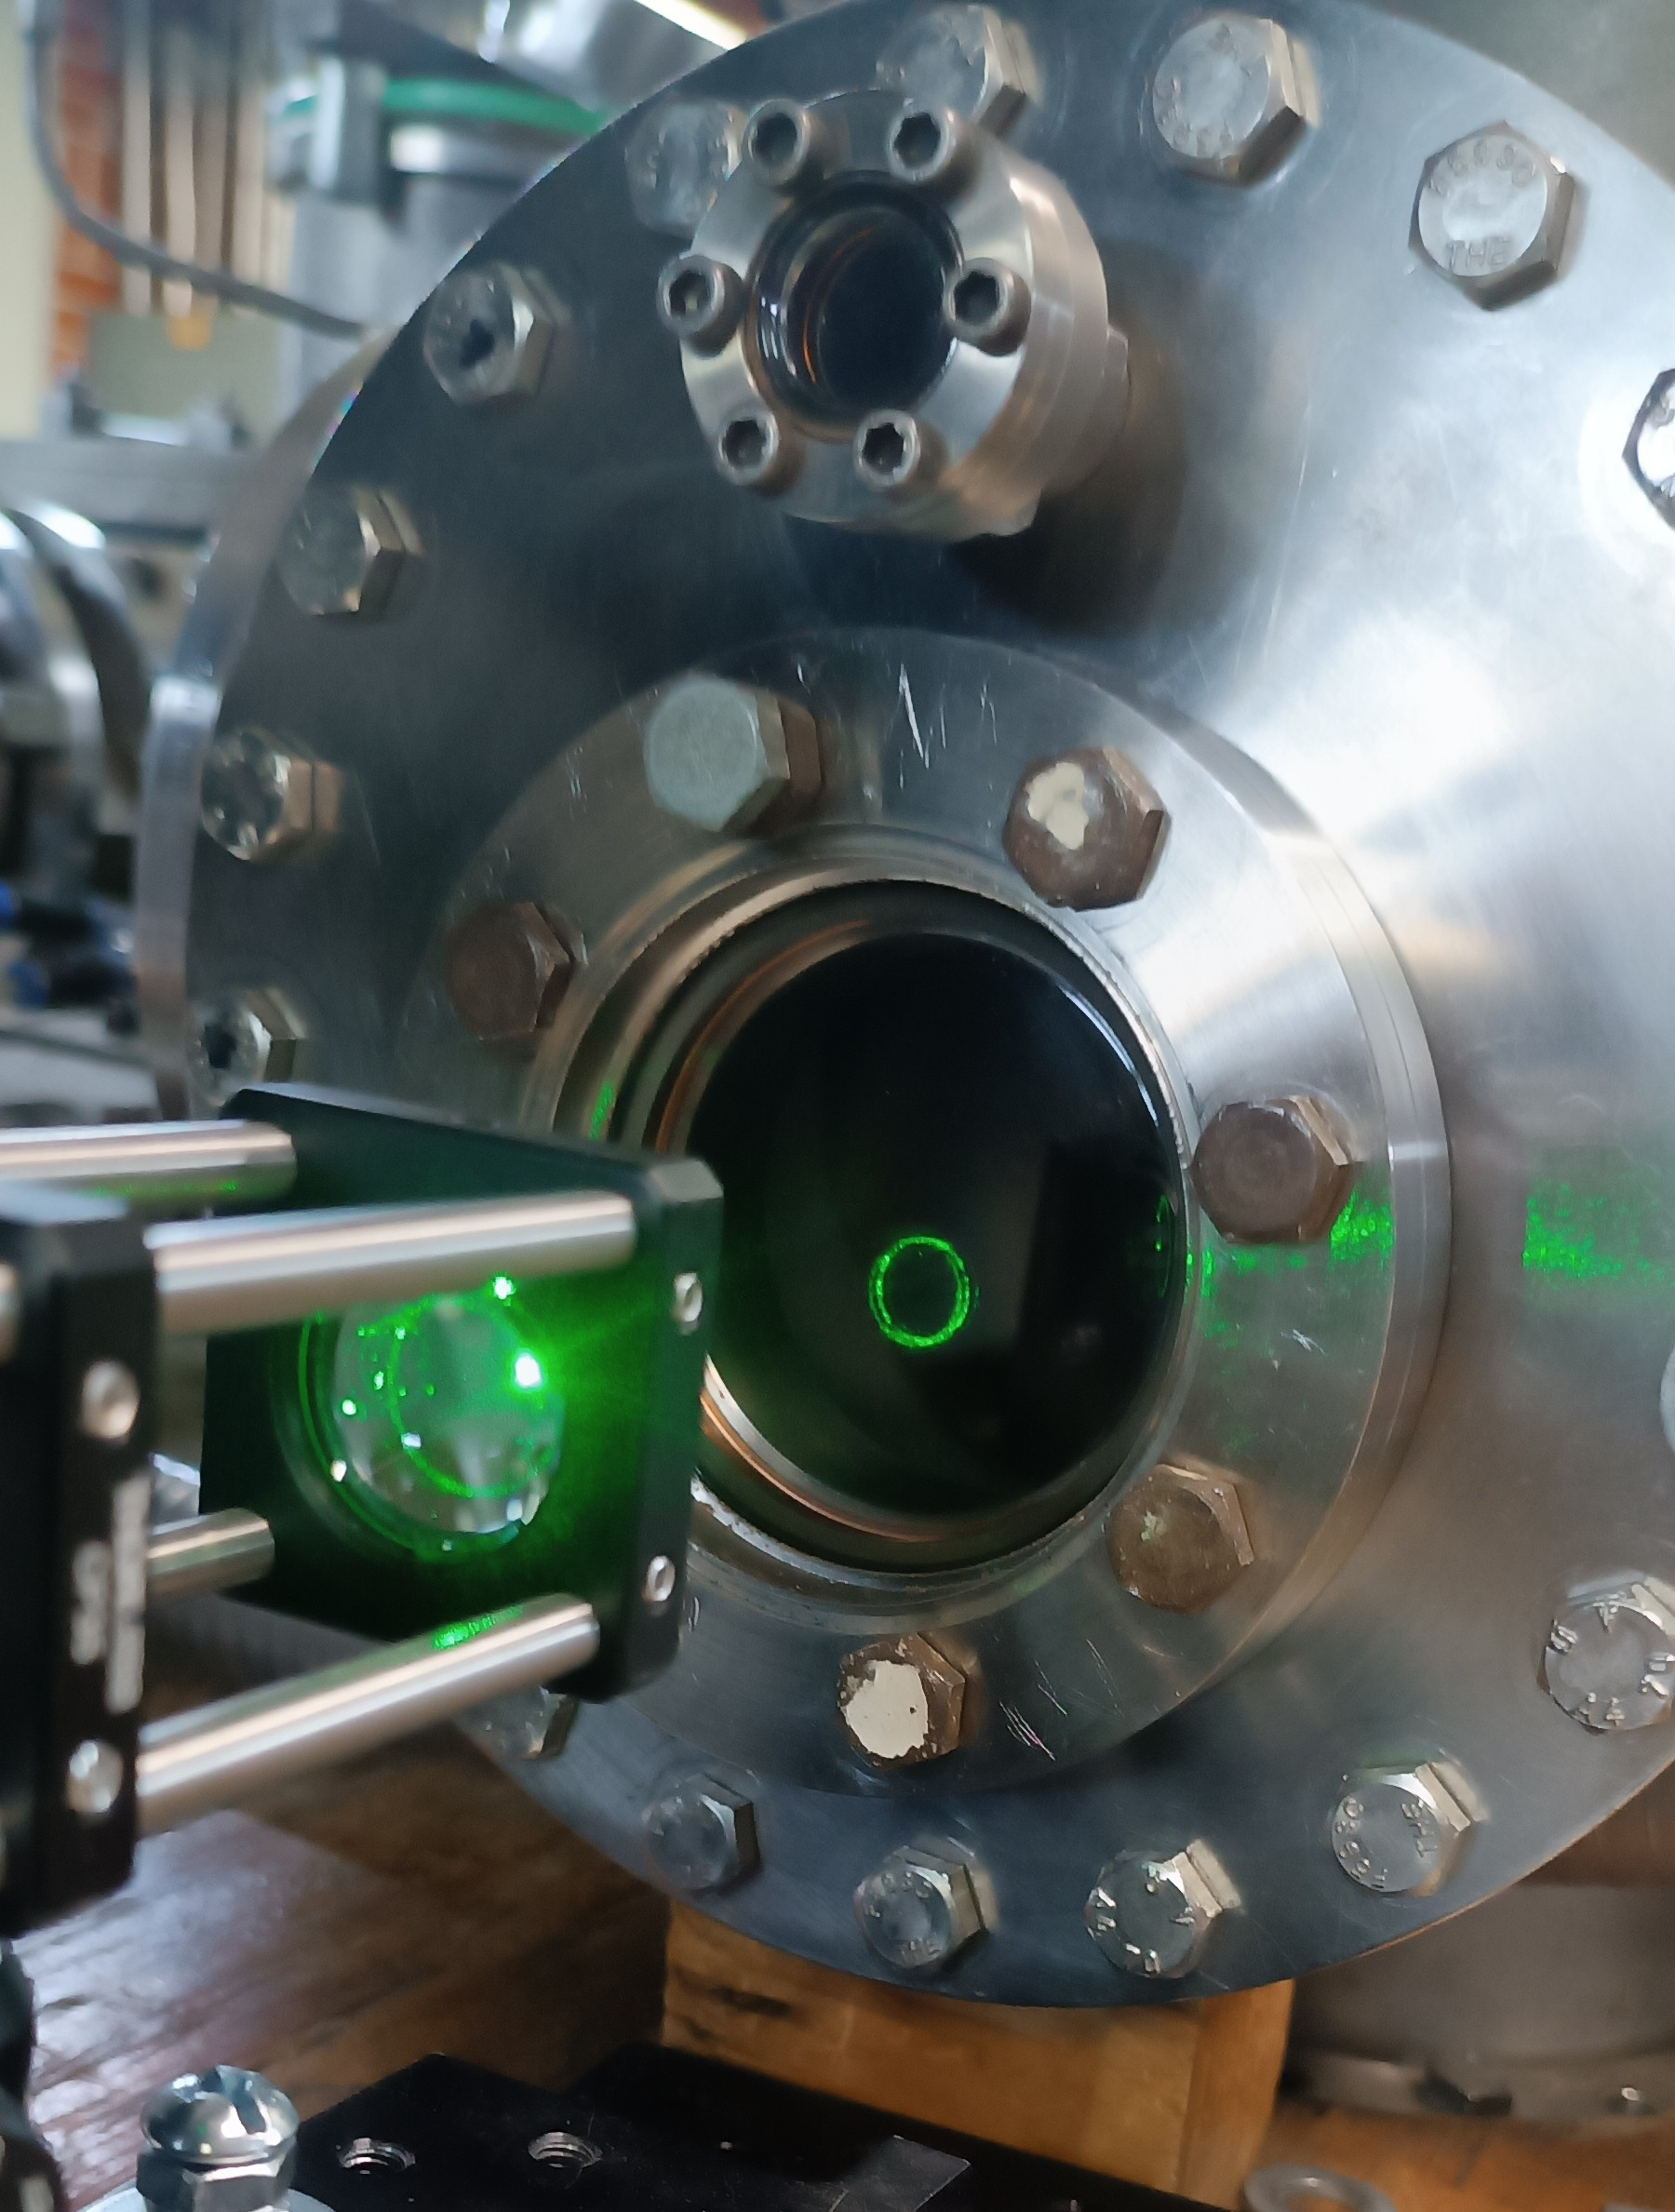
\includegraphics[width=0.6\linewidth]{figs/buenaaaaaaaaa.jpg}
	\caption{Espectrómetro óptico enfocado en la parte central del blanco de \ch{BN}.}
	\label{fig:Espectometro}
\end{figure}

\subsection{Medición de Espectros}

Para la medición de los espectros de emisión, este espectrómetro se colocó enfocado en el centro del blanco de nitruro de boro, a una altura de 5 cm por encima del mismo, este centro se vario cada 0.2 mm y se obtuvieron los datos respectivos de emisión, variando 2 cm a ambos lados de lo que se ubicó como el centro del blanco, la duración total del deposito fue de 20 minutos, dando por resultado el plasma que se se observa en \ref{fig:plasma}

\begin{figure}[htp]
	\centering
	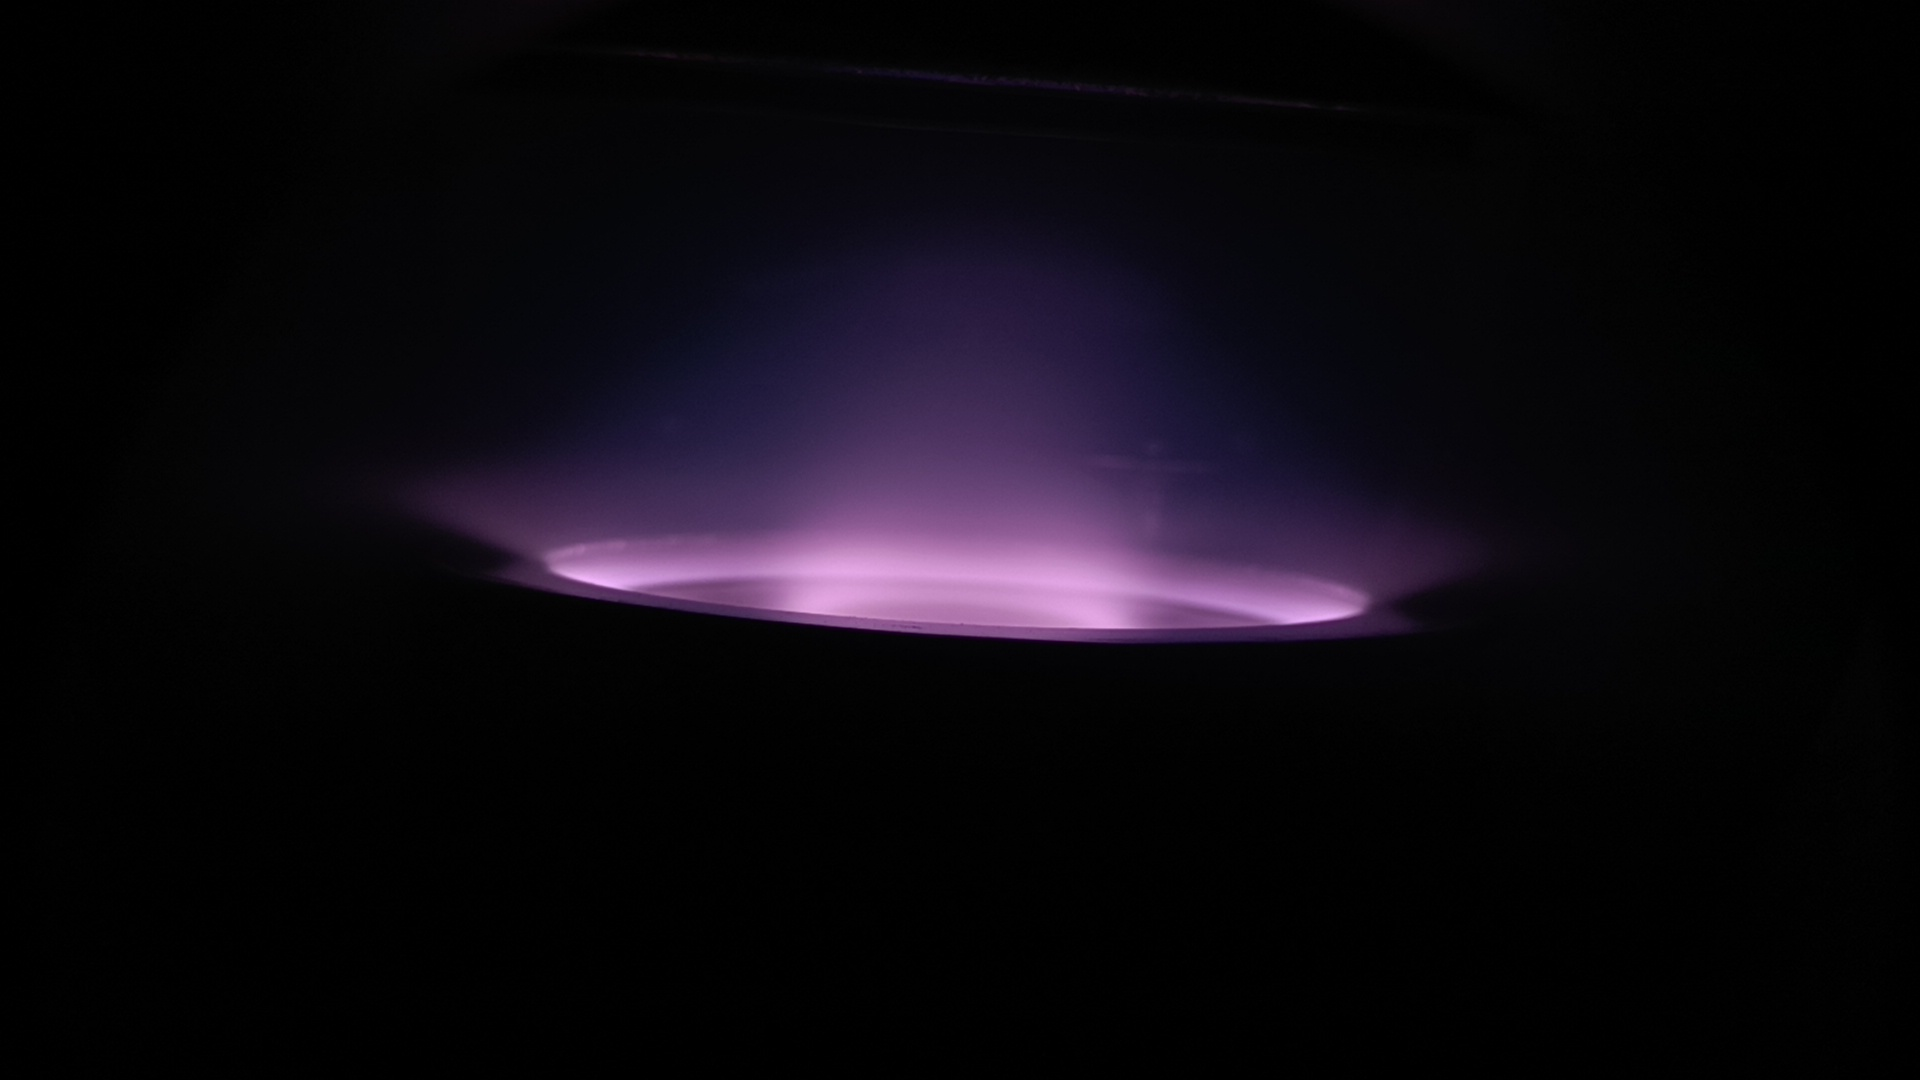
\includegraphics[width=0.8\linewidth]{PLASMA.jpg}
	\caption{Plasma generado durante el depósito de una película delgada de \ch{BN} mediante la técnica Rf.}
	\label{fig:plasma}
\end{figure}

\section{Resultados y análisis}

Una vez obtenida una gama de mediciones de los espectros de emisión  de diferentes posiciones alrededor del centro del blanco se procedió a comparar las lineas de emision obtenidas con las de National Institute of Standards and Technology Atomic Spectra Database, es importante aclarara que las longitudes de onda que captaba en espectometro optico variaba de $200 nm $ a $900 nm$.

\begin{figure}[htp]
	\centering
	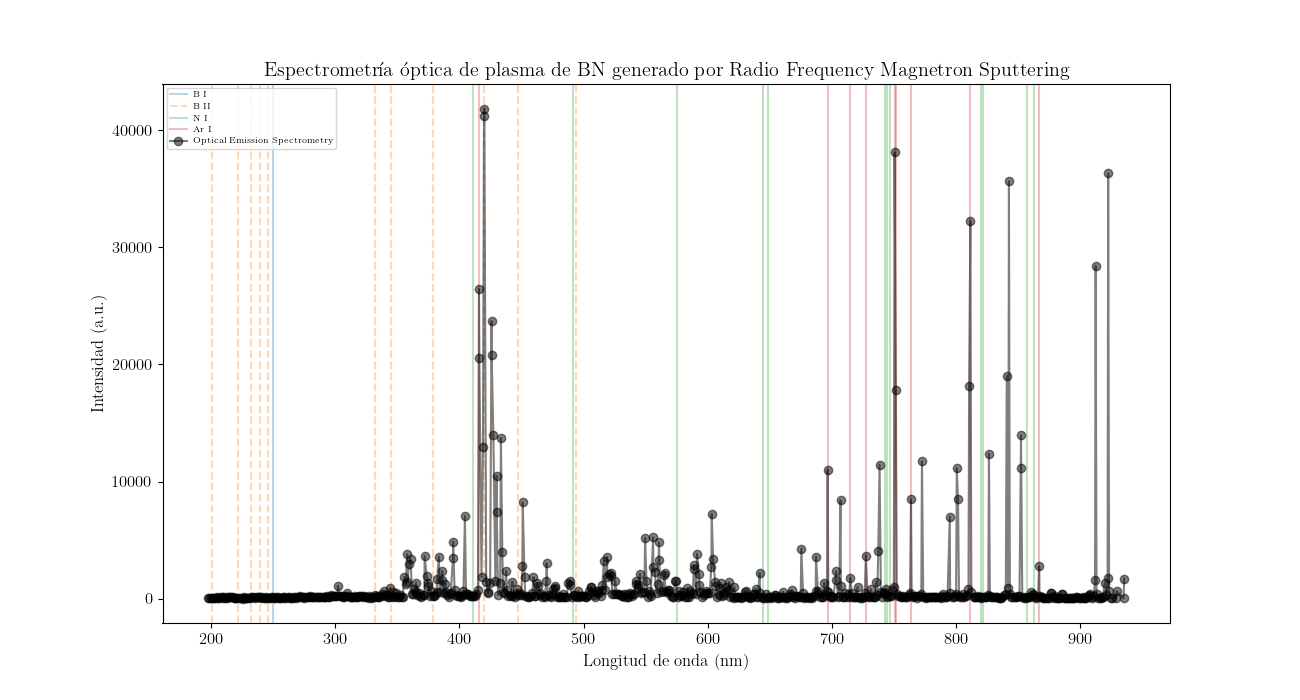
\includegraphics[width=0.9\linewidth]{figs/longitudes de onda.png}
	\caption{Comparacion de los espectros de emision teoricos y obtenidos en el laboratorio.}
	\label{Graf:plasma}
\end{figure}

Principalmente se identificaron las franjas de emisión de BI, BII, N y Ar, que es lo que esperaríamos del deposito encontrado, sin embargo, los datos obtenidos presentaban bastante ruido, esto se tomo en cuenta a la hora de filtrar, se esperaba encontrar otro elemento como el oxigeno, pues aunque este deposito se hace en una cámara de vacío, la extracción total del oxigeno presente en el aire es complicado de lograr, esto se le puede atribuir a movimientos en la mesa óptica y un cristal de la cámara de vació deteriorado pudieron afectar estas mediciones.


\section{Conclusiones}
El plasma es toda una área de la física por explorar y entender, se puede aprender bastante de su estudio para futuras aplicaciones principalmente en los temas relacionados con la Astrofísica, en este sentido al explorar los elementos en conjunto con un plasma generado nos

%%%%%%%%%%%%%%%%%%%%%%%%%%%%%%%%
%%%%%%    Bibliografia   %%%%%%%
%%%%%%%%%%%%%%%%%%%%%%%%%%%%%%%%
\nocite{*}
\printbibliography
\end{document}
